\documentclass[ignorenonframetext,]{beamer}
\setbeamertemplate{caption}[numbered]
\setbeamertemplate{caption label separator}{: }
\setbeamercolor{caption name}{fg=normal text.fg}
\beamertemplatenavigationsymbolsempty
\usepackage{lmodern}
\usepackage{amssymb,amsmath}
\usepackage{ifxetex,ifluatex}
\usepackage{fixltx2e} % provides \textsubscript
\ifnum 0\ifxetex 1\fi\ifluatex 1\fi=0 % if pdftex
  \usepackage[T1]{fontenc}
  \usepackage[utf8]{inputenc}
\else % if luatex or xelatex
  \ifxetex
    \usepackage{mathspec}
  \else
    \usepackage{fontspec}
  \fi
  \defaultfontfeatures{Ligatures=TeX,Scale=MatchLowercase}
\fi
\usetheme[]{CambridgeUS}
\usecolortheme{beaver}
\usefonttheme{structurebold}
% use upquote if available, for straight quotes in verbatim environments
\IfFileExists{upquote.sty}{\usepackage{upquote}}{}
% use microtype if available
\IfFileExists{microtype.sty}{%
\usepackage{microtype}
\UseMicrotypeSet[protrusion]{basicmath} % disable protrusion for tt fonts
}{}
\newif\ifbibliography
\hypersetup{
            pdftitle={A1 Erste Schritte mit R},
            pdfauthor={Jan-Philipp Kolb},
            pdfborder={0 0 0},
            breaklinks=true}
\urlstyle{same}  % don't use monospace font for urls
\usepackage{color}
\usepackage{fancyvrb}
\newcommand{\VerbBar}{|}
\newcommand{\VERB}{\Verb[commandchars=\\\{\}]}
\DefineVerbatimEnvironment{Highlighting}{Verbatim}{commandchars=\\\{\}}
% Add ',fontsize=\small' for more characters per line
\usepackage{framed}
\definecolor{shadecolor}{RGB}{248,248,248}
\newenvironment{Shaded}{\begin{snugshade}}{\end{snugshade}}
\newcommand{\KeywordTok}[1]{\textcolor[rgb]{0.13,0.29,0.53}{\textbf{#1}}}
\newcommand{\DataTypeTok}[1]{\textcolor[rgb]{0.13,0.29,0.53}{#1}}
\newcommand{\DecValTok}[1]{\textcolor[rgb]{0.00,0.00,0.81}{#1}}
\newcommand{\BaseNTok}[1]{\textcolor[rgb]{0.00,0.00,0.81}{#1}}
\newcommand{\FloatTok}[1]{\textcolor[rgb]{0.00,0.00,0.81}{#1}}
\newcommand{\ConstantTok}[1]{\textcolor[rgb]{0.00,0.00,0.00}{#1}}
\newcommand{\CharTok}[1]{\textcolor[rgb]{0.31,0.60,0.02}{#1}}
\newcommand{\SpecialCharTok}[1]{\textcolor[rgb]{0.00,0.00,0.00}{#1}}
\newcommand{\StringTok}[1]{\textcolor[rgb]{0.31,0.60,0.02}{#1}}
\newcommand{\VerbatimStringTok}[1]{\textcolor[rgb]{0.31,0.60,0.02}{#1}}
\newcommand{\SpecialStringTok}[1]{\textcolor[rgb]{0.31,0.60,0.02}{#1}}
\newcommand{\ImportTok}[1]{#1}
\newcommand{\CommentTok}[1]{\textcolor[rgb]{0.56,0.35,0.01}{\textit{#1}}}
\newcommand{\DocumentationTok}[1]{\textcolor[rgb]{0.56,0.35,0.01}{\textbf{\textit{#1}}}}
\newcommand{\AnnotationTok}[1]{\textcolor[rgb]{0.56,0.35,0.01}{\textbf{\textit{#1}}}}
\newcommand{\CommentVarTok}[1]{\textcolor[rgb]{0.56,0.35,0.01}{\textbf{\textit{#1}}}}
\newcommand{\OtherTok}[1]{\textcolor[rgb]{0.56,0.35,0.01}{#1}}
\newcommand{\FunctionTok}[1]{\textcolor[rgb]{0.00,0.00,0.00}{#1}}
\newcommand{\VariableTok}[1]{\textcolor[rgb]{0.00,0.00,0.00}{#1}}
\newcommand{\ControlFlowTok}[1]{\textcolor[rgb]{0.13,0.29,0.53}{\textbf{#1}}}
\newcommand{\OperatorTok}[1]{\textcolor[rgb]{0.81,0.36,0.00}{\textbf{#1}}}
\newcommand{\BuiltInTok}[1]{#1}
\newcommand{\ExtensionTok}[1]{#1}
\newcommand{\PreprocessorTok}[1]{\textcolor[rgb]{0.56,0.35,0.01}{\textit{#1}}}
\newcommand{\AttributeTok}[1]{\textcolor[rgb]{0.77,0.63,0.00}{#1}}
\newcommand{\RegionMarkerTok}[1]{#1}
\newcommand{\InformationTok}[1]{\textcolor[rgb]{0.56,0.35,0.01}{\textbf{\textit{#1}}}}
\newcommand{\WarningTok}[1]{\textcolor[rgb]{0.56,0.35,0.01}{\textbf{\textit{#1}}}}
\newcommand{\AlertTok}[1]{\textcolor[rgb]{0.94,0.16,0.16}{#1}}
\newcommand{\ErrorTok}[1]{\textcolor[rgb]{0.64,0.00,0.00}{\textbf{#1}}}
\newcommand{\NormalTok}[1]{#1}
\usepackage{graphicx,grffile}
\makeatletter
\def\maxwidth{\ifdim\Gin@nat@width>\linewidth\linewidth\else\Gin@nat@width\fi}
\def\maxheight{\ifdim\Gin@nat@height>\textheight0.8\textheight\else\Gin@nat@height\fi}
\makeatother
% Scale images if necessary, so that they will not overflow the page
% margins by default, and it is still possible to overwrite the defaults
% using explicit options in \includegraphics[width, height, ...]{}
\setkeys{Gin}{width=\maxwidth,height=\maxheight,keepaspectratio}

% Prevent slide breaks in the middle of a paragraph:
\widowpenalties 1 10000
\raggedbottom

\AtBeginPart{
  \let\insertpartnumber\relax
  \let\partname\relax
  \frame{\partpage}
}
\AtBeginSection{
  \ifbibliography
  \else
    \let\insertsectionnumber\relax
    \let\sectionname\relax
    \frame{\sectionpage}
  \fi
}
\AtBeginSubsection{
  \let\insertsubsectionnumber\relax
  \let\subsectionname\relax
  \frame{\subsectionpage}
}

\setlength{\parindent}{0pt}
\setlength{\parskip}{6pt plus 2pt minus 1pt}
\setlength{\emergencystretch}{3em}  % prevent overfull lines
\providecommand{\tightlist}{%
  \setlength{\itemsep}{0pt}\setlength{\parskip}{0pt}}
\setcounter{secnumdepth}{0}

\title{A1 Erste Schritte mit R}
\author{Jan-Philipp Kolb}
\date{11 Januar 2019}

\begin{document}
\frame{\titlepage}

\begin{frame}{Disclaimer/ Informationen vorab}

Normalerweise gibt es große Unterschiede bei Vorkenntnissen und
Fähigkeiten - bitte gebt Bescheid, wenn es zu schnell oder zu langsam
geht oder etwas unklar geblieben ist.

\begin{itemize}
\tightlist
\item
  Wenn es Fragen gibt - immer fragen
\item
  In diesem Kurs gibt es viele
  \href{http://web.math.ku.dk/~helle/R-intro/exercises.pdf}{\textbf{Übungen}},
  denn das Programmieren / die Nutzung von R lernt man am Ende nur
  allein.
\item
  Ich habe viele \href{https://www.showmeshiny.com/}{\textbf{Beispiele}}
  - probiert sie aus
\item
  R macht mehr Spaß zusammen - arbeitet zusammen!
\end{itemize}

\begin{block}{Motivation allgemein}

\begin{itemize}
\tightlist
\item
  Raumbezug herstellen/nutzen
\item
  Sekundäranalyse für bestehenden Daten
\item
  Analysepotentiale der Geokodierung vorstellen
\item
  Verbindung von sozial- mit raumwissenschaftlichen Daten
\end{itemize}

\end{block}

\begin{block}{Warum die Darstellung in Karten}

\begin{itemize}
\item
  Darstellung in Karten ermöglicht besseres Verständnis von
  sozialwissenschaftlicher Phänomene - Attraktiver Output
\item
  Durch die INSPIRE Richtlinie und \emph{Collaborative Mapping} wächst
  der verfügbare Bestand an Geodaten.
\item
  Daten sind oft frei verfügbar im Internet (z.B. Nutzung von APIs)
\item
  Die Daten sind oft wenig oder gar nicht strukturiert, heterogen und
  oft nicht zur räumlichen Visualisierung vorgesehen, beinhalten aber
  implizit geographische Informationen (Web 2.0)
\item
  Oftmals sind wenig oder keine Metadaten vorhanden
\end{itemize}

\end{block}

\end{frame}

\begin{frame}{Was heißt das für diesen Kurs}

\begin{block}{Vorgestellt werden:}

\begin{itemize}
\tightlist
\item
  Möglichkeiten für den Download, den Import, die Verarbeitung und die
  Visualisierung von Geodaten
\end{itemize}

\begin{itemize}
\item
  Quellen für Geodaten
\item
  Bspw. die wichtigsten Programmierschnittstellen (APIs) um die Daten zu
  bekommen
\item
  R-Pakete um diese Daten zu verarbeiten und zu visualisieren
\end{itemize}

\end{block}

\end{frame}

\begin{frame}{\href{https://www.ratswd.de/dl/downloads/RatSWD_Geodatenbericht.pdf}{Das
Thema Geodatenlandschaft}}


\includegraphics{figure/BildRatSWDBericht.png}

\end{frame}

\begin{frame}{Gründe R zu nutzen\ldots{}}

\begin{itemize}
\item
  \ldots{} R ist eine
  \href{https://stackoverflow.com/questions/1546583/what-is-the-definition-of-an-open-source-programming-language}{\textbf{quelloffene
  Sprache}}
\item
  \ldots{} hervorragende
  \href{http://matthewlincoln.net/2014/12/20/adjacency-matrix-plots-with-r-and-ggplot2.html}{\textbf{Grafiken}},
  \href{https://www.r-bloggers.com/3d-plots-with-ggplot2-and-plotly\%20/}{\textbf{Grafiken}},
  \href{https://procomun.wordpress.com/2011/03/18/splomr/}{\textbf{Grafiken}}
\item
  \ldots{} \href{https://github.com/Japhilko/RInterfaces}{\textbf{R kann
  in Kombination mit anderen Programmen verwendet werden}} - z.B. zur
  \href{https://github.com/Japhilko/RInterfaces/blob/master/slides/Datenimport.md}{\textbf{Verknüpfung
  von Daten}}
\item
  \ldots{} R kann
  \href{https://cran.r-project.org/web/packages/MplusAutomation/index.html}{\textbf{zur
  Automatisierung}} verwendet werden
\item
  \ldots{} Breite und aktive Community -
  \href{https://www.r-bloggers.com/}{\textbf{Man kann die Intelligenz
  anderer Leute nutzen ;-)}}
\end{itemize}

\end{frame}

\begin{frame}{R kann in Kombination mit anderen Programmen genutzt
werden\ldots{}}

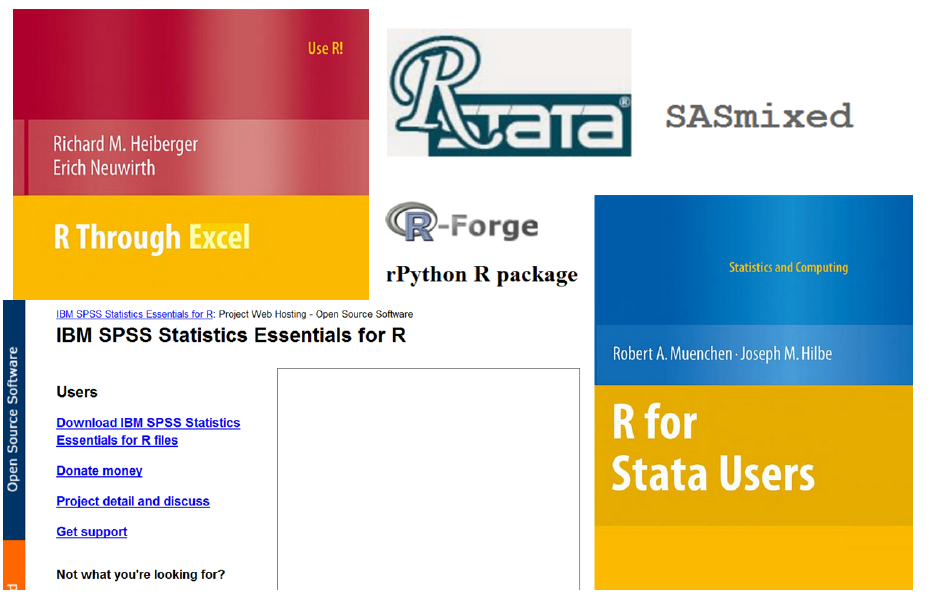
\includegraphics{figure/Rinterfaces.PNG}

\begin{itemize}
\tightlist
\item
  Schnittstelle zu:
  \href{https://cran.r-project.org/web/packages/reticulate/vignettes/calling_python.html}{\textbf{Python}},
  \href{https://www.springer.com/de/book/9781441900517}{\textbf{Excel}},
  \href{https://www.ibm.com/support/knowledgecenter/en/SSFUEU_7.2.0/com.ibm.swg.ba.cognos.op_capmod_ig.7.2.0.doc/t_essentials_for_r_statistics.html}{\textbf{SPSS}},
  \href{https://cran.r-project.org/web/packages/SASmixed/index.html}{\textbf{SAS}},
  \href{https://cran.r-project.org/web/packages/RStata/index.html}{\textbf{Stata}}
\end{itemize}

\end{frame}

\begin{frame}{\href{https://gallery.shinyapps.io/cran-gauge/}{\textbf{Die
Beliebtheit von R-Paketen}}}

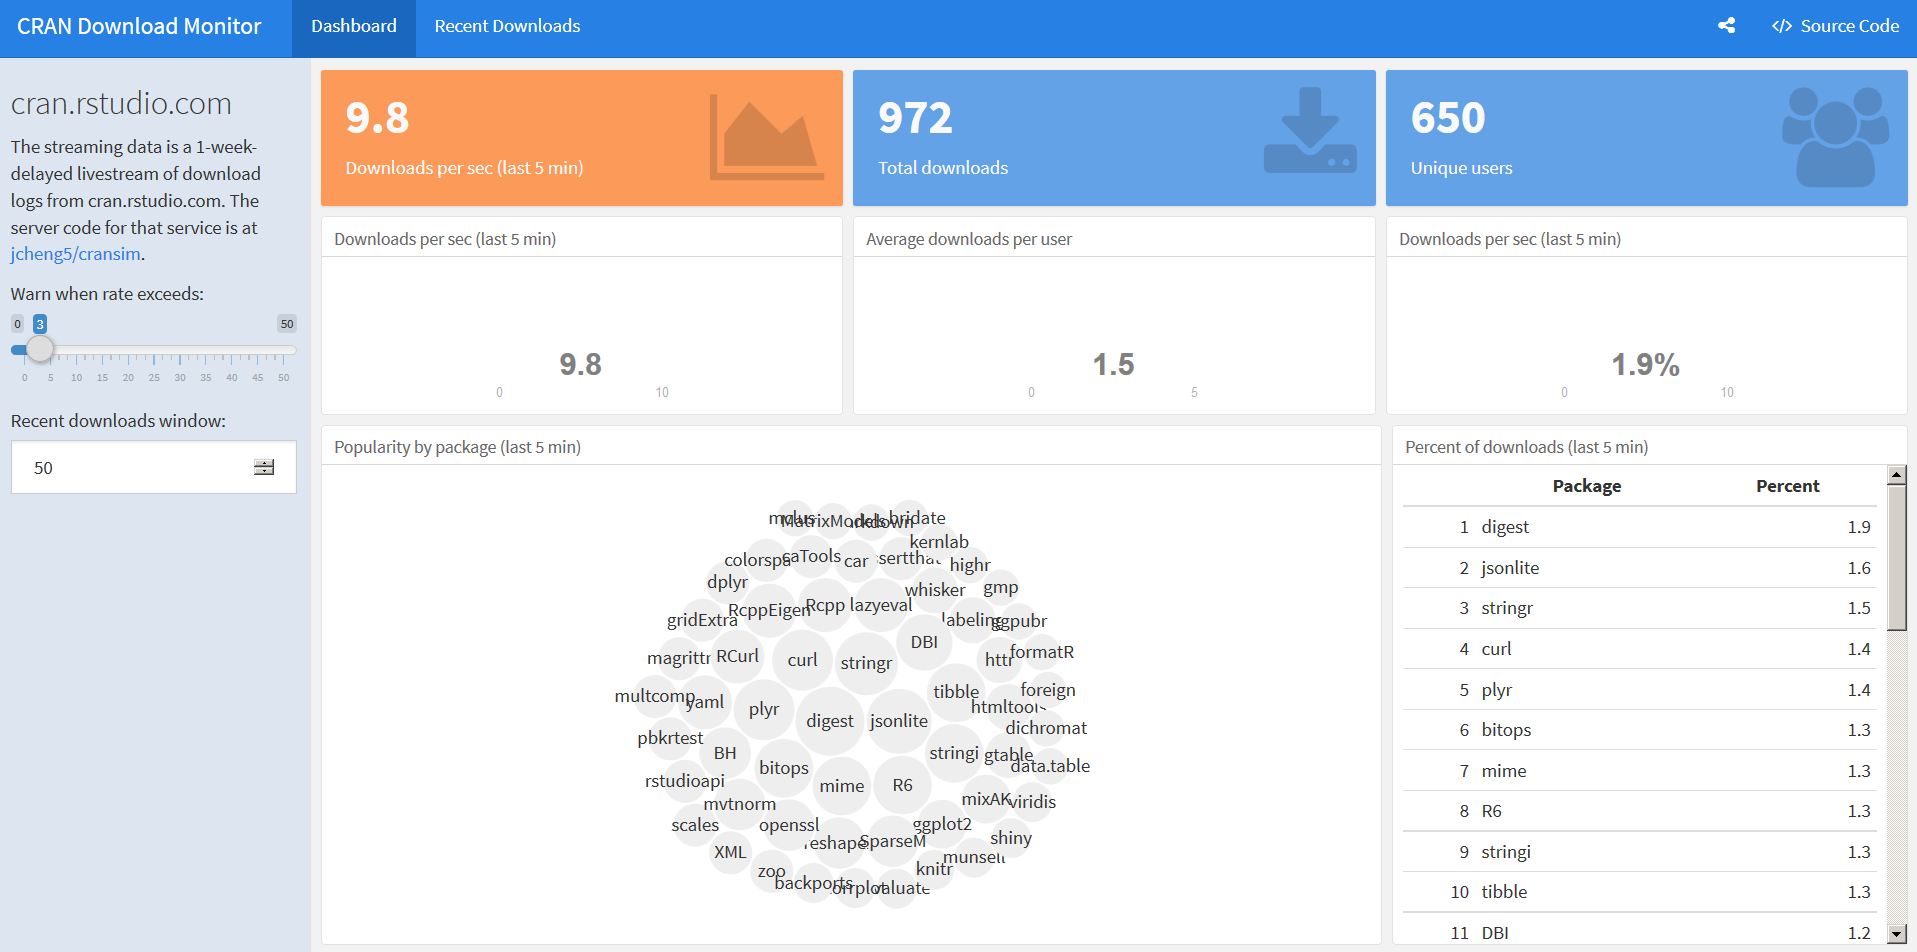
\includegraphics{figure/CRANdownloads.PNG}

\end{frame}

\begin{frame}{Download R:}

\url{http://www.r-project.org/}

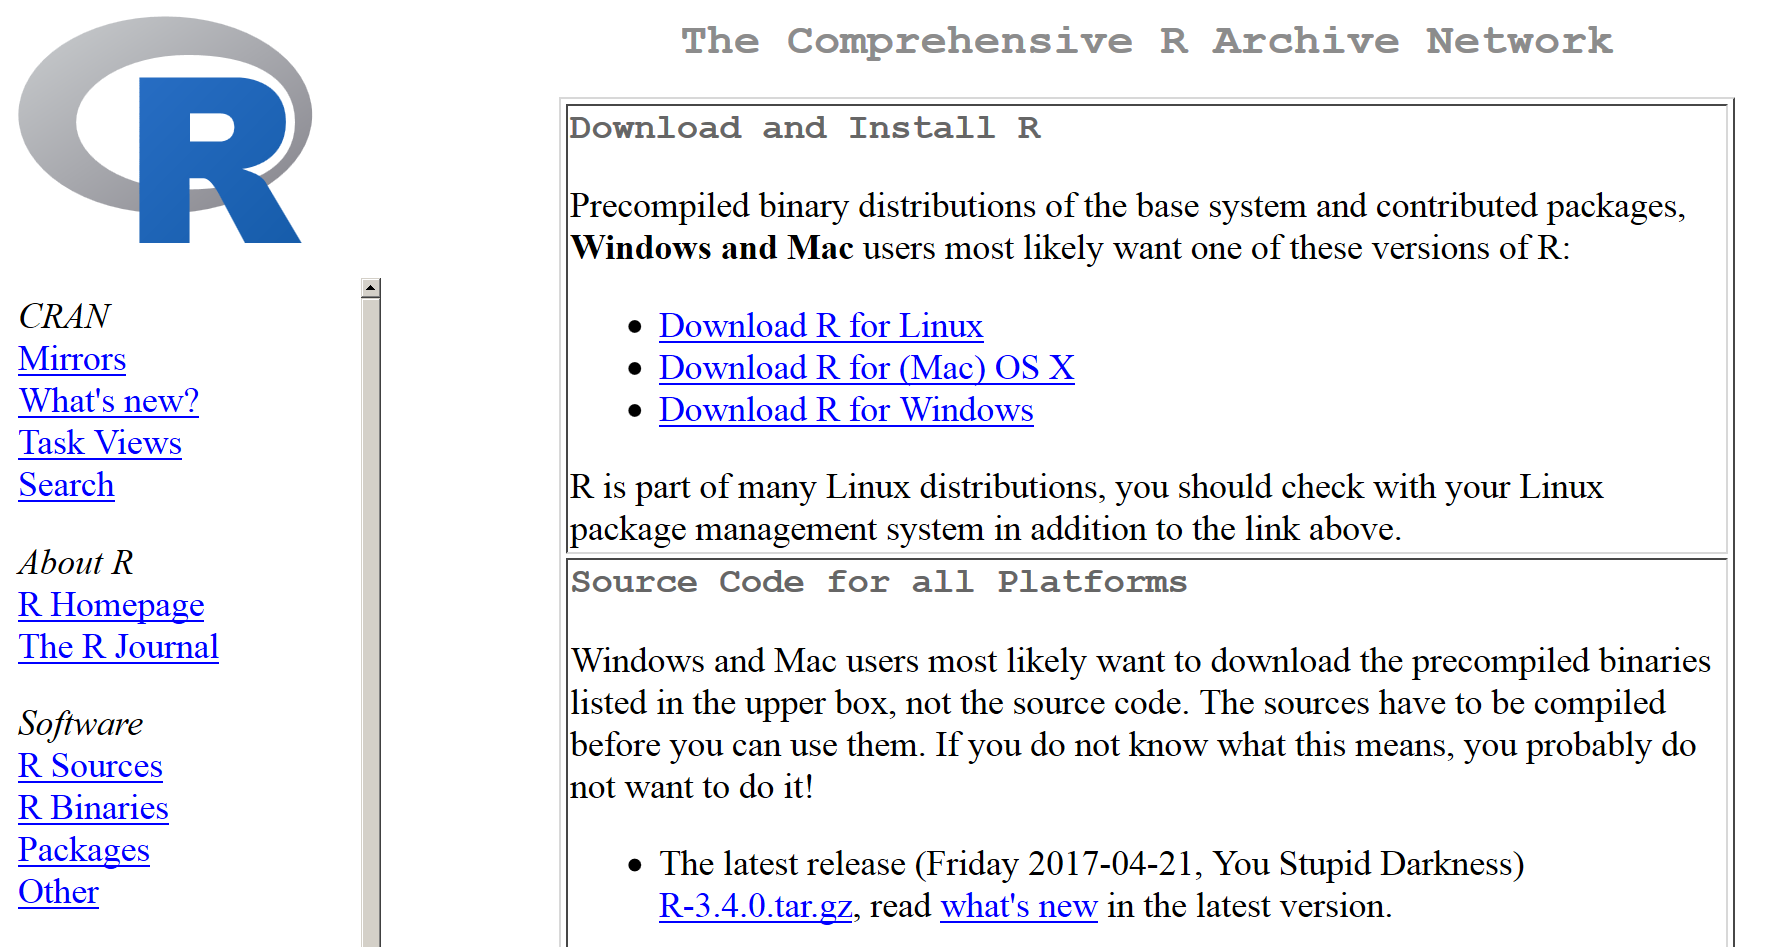
\includegraphics{figure/CRAN1picture.PNG}

\end{frame}

\begin{frame}{Open Source Programm R}

\begin{block}{Das ist das Basis-R:}

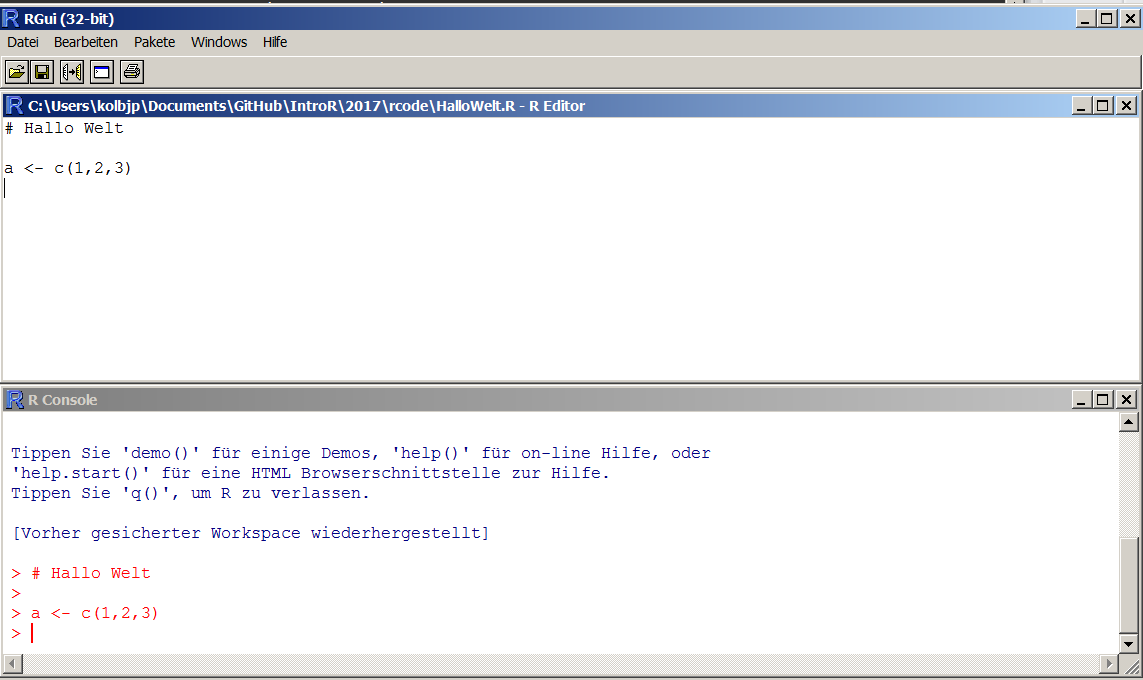
\includegraphics{figure/BasisR.PNG}

\end{block}

\end{frame}

\begin{frame}{Graphical user interface}

Viele Leute nutzen ein
\href{https://en.wikipedia.org/wiki/Graphical_user_interface}{\textbf{Graphical
User Interface}} (GUI) oder ein
\href{https://en.wikipedia.org/wiki/Integrated_development_environment}{\textbf{Integrated
Development Interface}} (IDE).

Aus den folgenden Gründen:

\begin{itemize}
\tightlist
\item
  Syntax-Hervorhebung
\item
  Auto-Vervollständigung
\item
  Bessere Übersicht über Graphiken, Pakete, Dateien, \ldots{}
\end{itemize}

\end{frame}

\begin{frame}{RStudio}

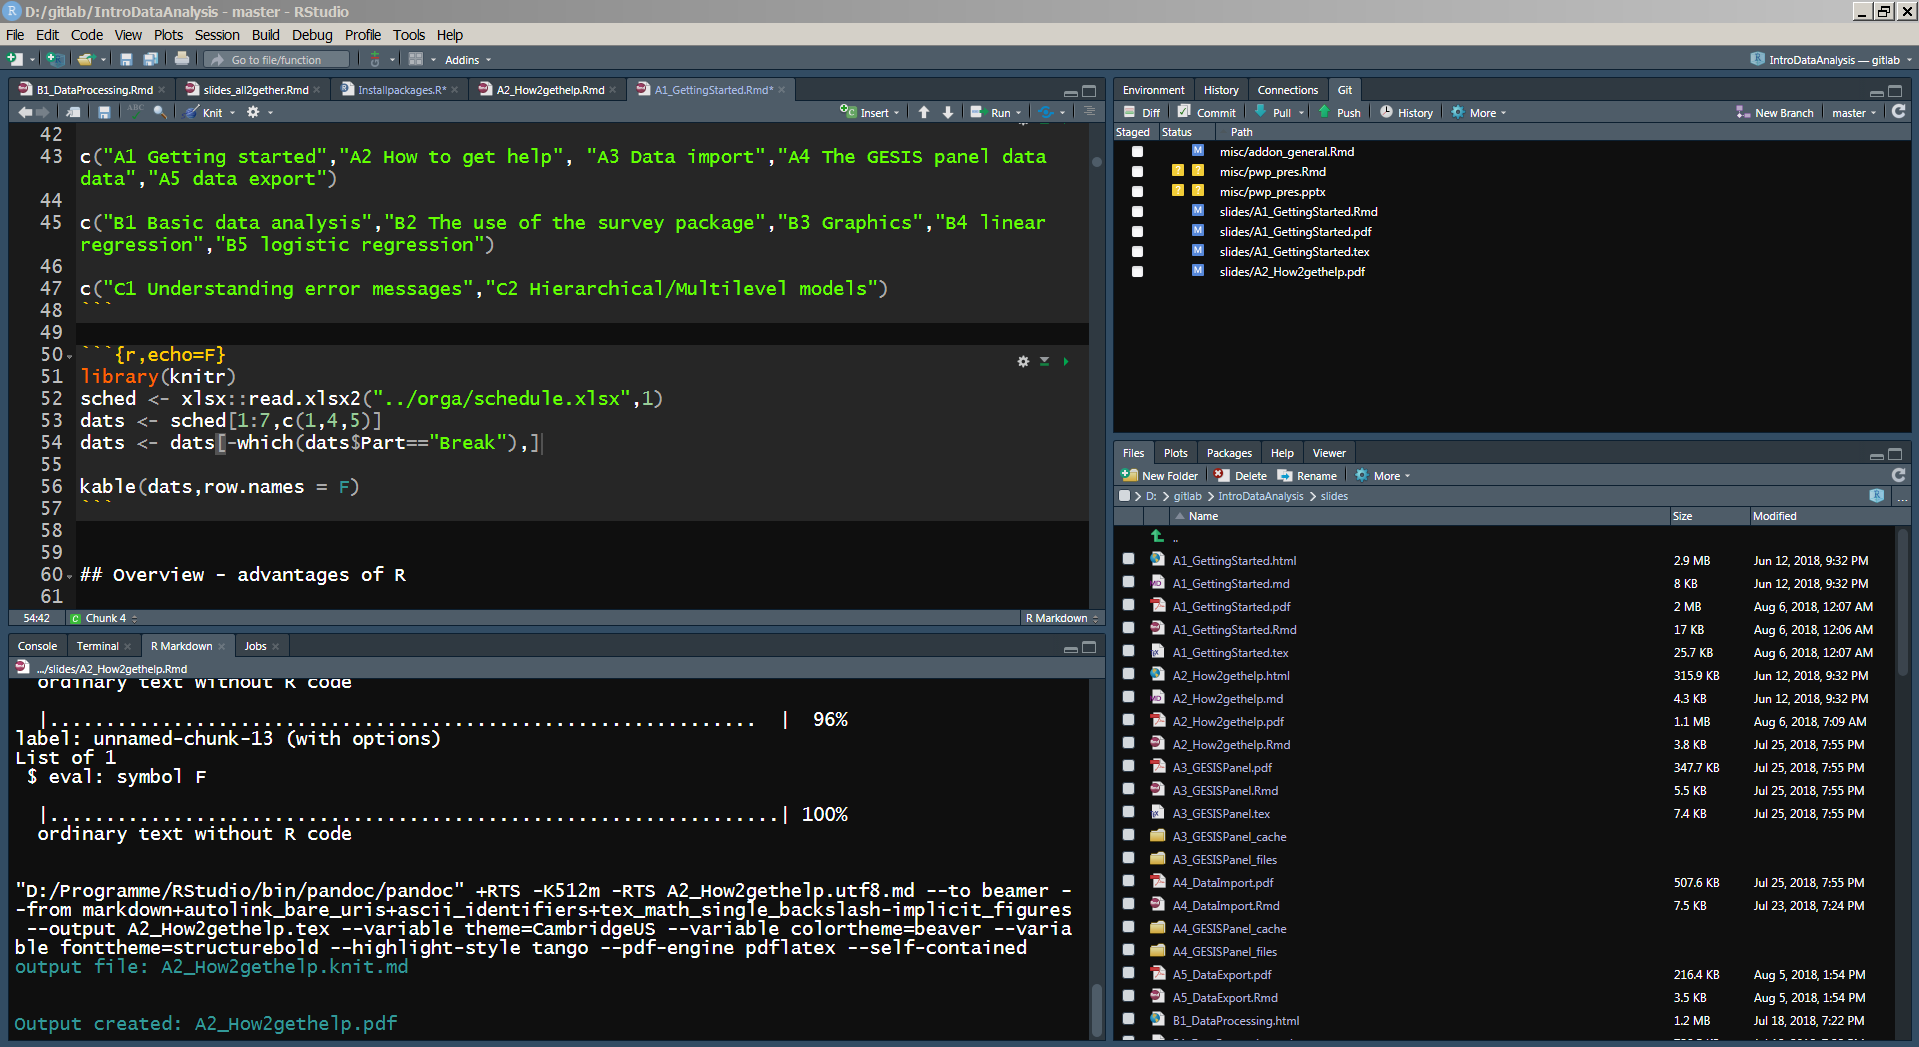
\includegraphics{figure/RstudioExample.PNG}

\end{frame}

\begin{frame}[fragile]{A1A Übung - Vorbereitung}

\begin{itemize}
\tightlist
\item
  Schaue, ob R auf dem Computer installiert ist
\item
  Wenn nicht, lade \href{r-project.org}{\textbf{R}} herunter und
  installiere es.
\item
  Prüfe ob Rstudio installiert ist.
\item
  Wenn nicht - \href{http://www.rstudio.com/}{\textbf{installiere}}
  Rstudio.
\item
  Starte RStudio. Gehe in die Konsole (meistens Fenster unten links) und
  tippe
\end{itemize}

\begin{Shaded}
\begin{Highlighting}[]
\DecValTok{3}\OperatorTok{+}\DecValTok{2}
\end{Highlighting}
\end{Shaded}

\begin{itemize}
\tightlist
\item
  Wenn noch kein Skript geöffnet im oberen linken Teil von Rstudio
  geöffnet ist, gehe zum Menü und öffne ein neues Skript. Checks das
  Datum mit \texttt{date()} und die R version mit
  \texttt{sessionInfo()}.
\end{itemize}

\begin{Shaded}
\begin{Highlighting}[]
\KeywordTok{date}\NormalTok{()}
\end{Highlighting}
\end{Shaded}

\begin{Shaded}
\begin{Highlighting}[]
\KeywordTok{sessionInfo}\NormalTok{()}
\end{Highlighting}
\end{Shaded}

\end{frame}

\begin{frame}[fragile]{R ist eine objektorientierte Sprache.}

\begin{block}{Vektoren und Zuweisungen}

\begin{itemize}
\tightlist
\item
  \texttt{\textless{}-} ist der Zuweisungsoperator
\end{itemize}

\begin{Shaded}
\begin{Highlighting}[]
\NormalTok{b <-}\StringTok{ }\KeywordTok{c}\NormalTok{(}\DecValTok{1}\NormalTok{,}\DecValTok{2}\NormalTok{) }\CommentTok{# create an object with the numbers 1 and 2}
\end{Highlighting}
\end{Shaded}

\begin{itemize}
\tightlist
\item
  Auf dieses Objekt kann eine Funktion angewendet werden:
\end{itemize}

\begin{Shaded}
\begin{Highlighting}[]
\KeywordTok{mean}\NormalTok{(b) }\CommentTok{# computes the mean}
\end{Highlighting}
\end{Shaded}

\begin{verbatim}
## [1] 1.5
\end{verbatim}

Mit diesen Funktionen können wir etwas über die Eigenschaften des
Objekts erfahren:

\begin{Shaded}
\begin{Highlighting}[]
\KeywordTok{length}\NormalTok{(b) }\CommentTok{# b has the length 2}
\end{Highlighting}
\end{Shaded}

\begin{verbatim}
## [1] 2
\end{verbatim}

\end{block}

\begin{block}{Objektstruktur}

\begin{Shaded}
\begin{Highlighting}[]
\KeywordTok{str}\NormalTok{(b) }\CommentTok{# b is a numeric vector}
\end{Highlighting}
\end{Shaded}

\begin{verbatim}
##  num [1:2] 1 2
\end{verbatim}

\end{block}

\end{frame}

\begin{frame}[fragile]{A1B Übung - Zuweisungen und Funktionen}

Erstellen Sie einen Vektor \texttt{b} mit den Zahlen von 1 bis 5 und
berechnen Sie\ldots{}.

\begin{enumerate}
\def\labelenumi{\arabic{enumi}.}
\item
  den Mittelwert
\item
  die Varianz
\item
  die Standardabweichung
\item
  die Quadratwurzel aus dem Mittelwert
\end{enumerate}

\end{frame}

\begin{frame}{\href{https://stats.idre.ucla.edu/r/seminars/intro/}{\textbf{Wo
man Routinen findet}}}

\begin{itemize}
\tightlist
\item
  Viele Funktionen sind in Basis-R enthalten.
\item
  Viele spezifische Funktionen sind in zusätzliche Bibliotheken
  integriert.
\item
  R kann modular durch sogenannte Pakete oder Bibliotheken erweitert
  werden.
\item
  Die wichtigsten Pakete, die auf CRAN gehostet werden (13481 at Fr Dez
  07)
\item
  Weitere Pakete findet man z.B. unter
  \href{www.bioconductor.org}{\textbf{bioconductor}}
\end{itemize}

\end{frame}

\begin{frame}{\href{https://www.youtube.com/watch?v=kKI9--Opmso}{Übersicht
R-Pakete}}

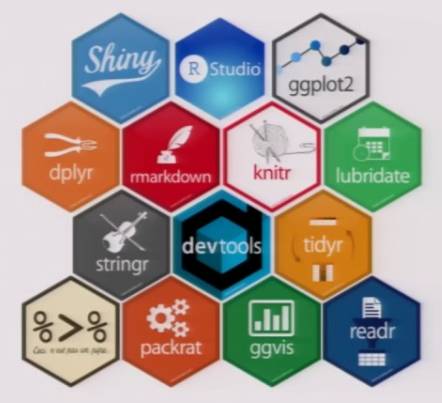
\includegraphics{figure/packages_overview.PNG}

\end{frame}

\begin{frame}[fragile]{Installation von Paketen}

\begin{itemize}
\tightlist
\item
  Die Anführungszeichen um den Paketnamen herum sind für den Befehl
  \texttt{install.packages} notwendig.
\item
  Sie sind optional für den Befehl \texttt{library}.
\item
  Man kann auch \texttt{require} anstelle von \texttt{library}
  verwenden.
\end{itemize}

\begin{Shaded}
\begin{Highlighting}[]
\KeywordTok{install.packages}\NormalTok{(}\StringTok{"raster"}\NormalTok{)}

\KeywordTok{library}\NormalTok{(raster)}
\end{Highlighting}
\end{Shaded}

\end{frame}

\begin{frame}{Installation von Paketen mit RStudio}

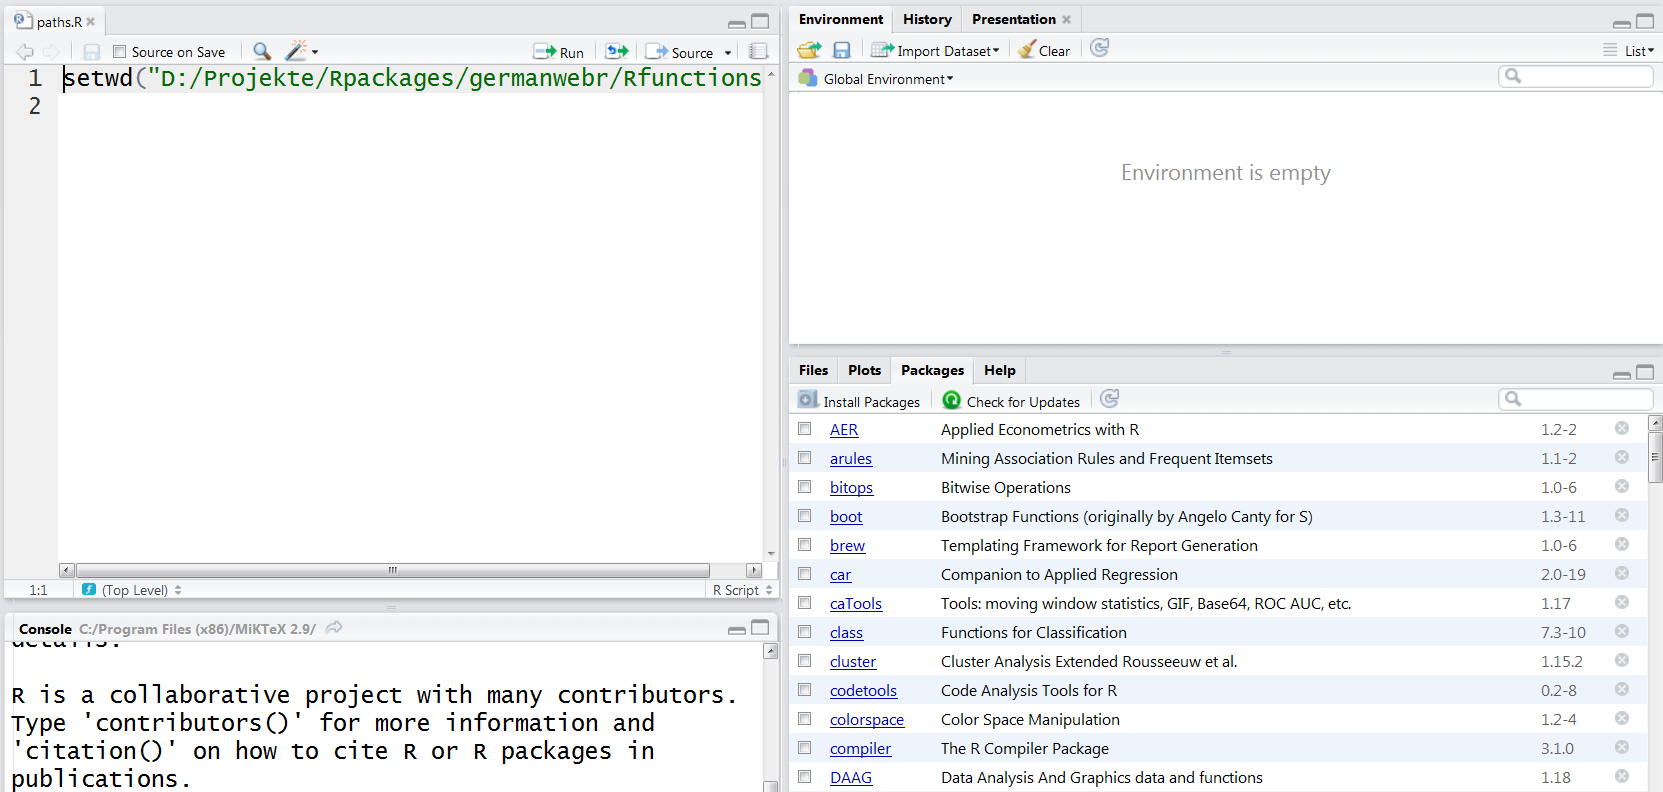
\includegraphics{figure/PaketeRstudio.PNG}

\end{frame}

\begin{frame}{Bestehende Pakete und Installation}

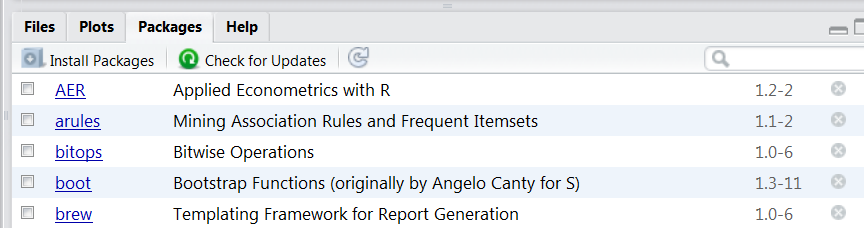
\includegraphics{figure/packages3.PNG}

\end{frame}

\begin{frame}[fragile]{Übersicht über viele nützliche Pakete:}

\begin{itemize}
\tightlist
\item
  Luhmann -
  \href{http://www.beltz.de/fileadmin/beltz/downloads/OnlinematerialienPVU/28090_Luhmann/Verwendete\%20Pakete.pdf}{\textbf{Übersicht
  mit vielen nützlichen Paketen}}
\end{itemize}

\begin{block}{Weitere interessante Pakete:}

\begin{itemize}
\tightlist
\item
  Das Paket \texttt{sf} - bietet Zugang zu
  \href{https://de.wikipedia.org/wiki/Simple_Feature_Access}{\textbf{simple
  features}}.
\item
  Mit dem Paket \texttt{leaflet} kann man interaktive Karten erstellen.
\item
  Das Paket \texttt{tmap} kann zur Erstellung von thematischen Karten
  genutzt werden.
\item
  \href{http://www.r-bloggers.com/tag/maptools/}{\textbf{Paket
  \texttt{maptools} um Karten zu erzeugen}}
\end{itemize}


\includegraphics{figure/logo_sf.PNG}

\end{block}

\end{frame}

\begin{frame}[fragile]{Pakete aus verschiedenen Quellen installieren}

\begin{block}{Pakete vom CRAN Server installieren}

\begin{Shaded}
\begin{Highlighting}[]
\KeywordTok{install.packages}\NormalTok{(}\StringTok{"lme4"}\NormalTok{)}
\end{Highlighting}
\end{Shaded}

\end{block}

\begin{block}{Pakete vom Bioconductor Server installieren}

\begin{Shaded}
\begin{Highlighting}[]
\KeywordTok{source}\NormalTok{(}\StringTok{"https://bioconductor.org/biocLite.R"}\NormalTok{)}
\KeywordTok{biocLite}\NormalTok{(}\KeywordTok{c}\NormalTok{(}\StringTok{"GenomicFeatures"}\NormalTok{, }\StringTok{"AnnotationDbi"}\NormalTok{))}
\end{Highlighting}
\end{Shaded}

\end{block}

\begin{block}{Pakete von Github installieren}

\begin{Shaded}
\begin{Highlighting}[]
\KeywordTok{install.packages}\NormalTok{(}\StringTok{"devtools"}\NormalTok{)}
\KeywordTok{library}\NormalTok{(devtools)}

\KeywordTok{install_github}\NormalTok{(}\StringTok{"hadley/maptools"}\NormalTok{)}
\end{Highlighting}
\end{Shaded}

\end{block}

\end{frame}

\begin{frame}{Wie bekomme ich einen Überblick?}

\begin{itemize}
\item
  Entdecke Pakete, die kürzlich auf den
  \href{https://mran.microsoft.com/packages/}{\textbf{CRAN}} Server
  hochgeladen wurden
\item
  Nutze eine Shiny Web-App, die
  \href{https://gallery.shinyapps.io/cran-gauge/}{\textbf{Pakete
  anzeigt, die kürzlich von CRAN}} heruntergeladen wurden.
\item
  Werfe einen Blick auf eine
  \href{https://support.rstudio.com/hc/en-us/articles/201057987-Quick-list-of-useful-R-packages}{\textbf{Quick-Liste
  nützlicher Pakete}}
\item
  \ldots{}., oder auf eine Liste mit den
  \href{http://www.computerworld.com/article/2921176/business-intelligence/great-r-packages-for-data-import-wrangling-visualization.html}{\textbf{besten
  Paketen für die Datenverarbeitung und -analyse}},\ldots{}..
\item
  \ldots{}., oder schaue unter
  \href{https://www.r-bloggers.com/the-50-most-used-r-packages/}{\textbf{die
  50 meistgenutzten Pakete}}
\end{itemize}

\end{frame}

\begin{frame}[fragile]{CRAN Task Views}

\begin{itemize}
\tightlist
\item
  Bezüglich mancher Themen gibt es einen Überblick über alle wichtigen
  Pakete - (\href{https://cran.r-project.org/web/views/}{\textbf{CRAN
  Task Views}})
\item
  Momentan gibt es 35 Task Views.
\item
  Alle Pakete einer Task-View können mit folgendem Befehl installiert
  werden:
  \href{https://mran.microsoft.com/rpackages/}{\textbf{command:}}
\end{itemize}

\begin{Shaded}
\begin{Highlighting}[]
\KeywordTok{install.packages}\NormalTok{(}\StringTok{"ctv"}\NormalTok{)}
\KeywordTok{library}\NormalTok{(}\StringTok{"ctv"}\NormalTok{)}
\KeywordTok{install.views}\NormalTok{(}\StringTok{"Spatial"}\NormalTok{)}
\end{Highlighting}
\end{Shaded}

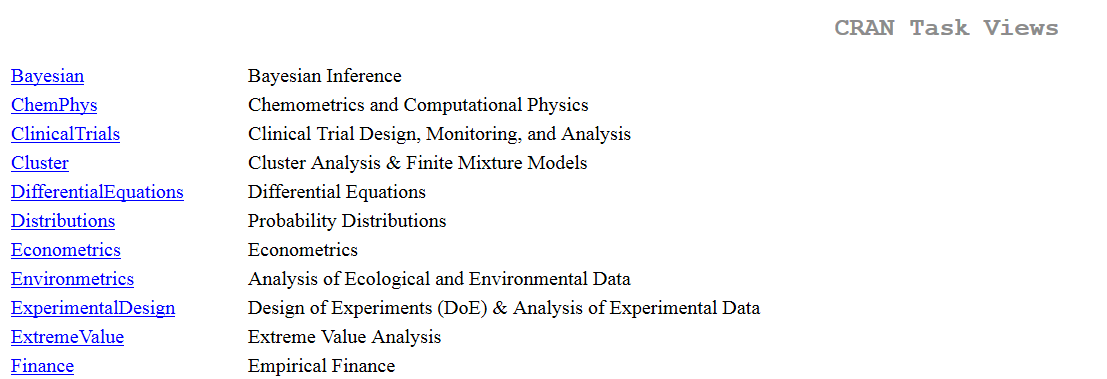
\includegraphics{figure/CRANtaskViews.PNG}

\end{frame}

\begin{frame}{A1C Übung - zusätzliche Pakete}

Geh bspw. auf \url{https://cran.r-project.org/} und suche nach
Paketen\ldots{}

\begin{itemize}
\tightlist
\item
  die sich für interaktive Karten eignen.
\item
  mit denen man thematische Karten erstellen kann
\item
  mit denen man die räumliche Distanz berechnen kann
\item
  mit denen man eine Satelitenkarte bekommen kann
\end{itemize}

\end{frame}

\begin{frame}{Robin Lovelace -
\href{https://geocompr.robinlovelace.net/}{Geocomputation with R}}


\includegraphics{figure/cover_lovelace.png}

\end{frame}

\begin{frame}{Typen von
\href{https://geocompr.robinlovelace.net/spatial-class.html}{simple
feature die von \texttt{sf} unterstützt werden.}}

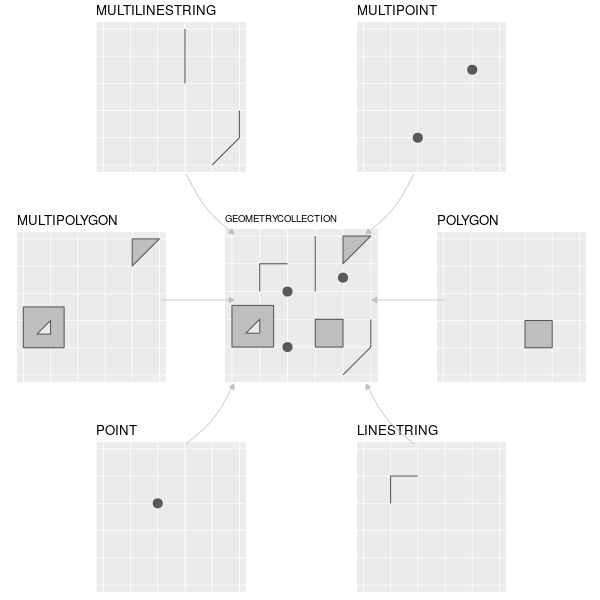
\includegraphics{figure/sf-classes.png}

\end{frame}

\begin{frame}[fragile]{Erste Weltkarten}

\begin{Shaded}
\begin{Highlighting}[]
\KeywordTok{library}\NormalTok{(sf)}
\end{Highlighting}
\end{Shaded}

\begin{verbatim}
## Linking to GEOS 3.6.1, GDAL 2.2.3, PROJ 4.9.3
\end{verbatim}

\begin{Shaded}
\begin{Highlighting}[]
\KeywordTok{library}\NormalTok{(spData) }
\end{Highlighting}
\end{Shaded}

\begin{verbatim}
## To access larger datasets in this package, install the spDataLarge
## package with: `install.packages('spDataLarge',
## repos='https://nowosad.github.io/drat/', type='source')`
\end{verbatim}

\begin{Shaded}
\begin{Highlighting}[]
\KeywordTok{plot}\NormalTok{(world)}
\end{Highlighting}
\end{Shaded}

\begin{verbatim}
## Warning: plotting the first 9 out of 10 attributes; use max.plot = 10 to
## plot all
\end{verbatim}

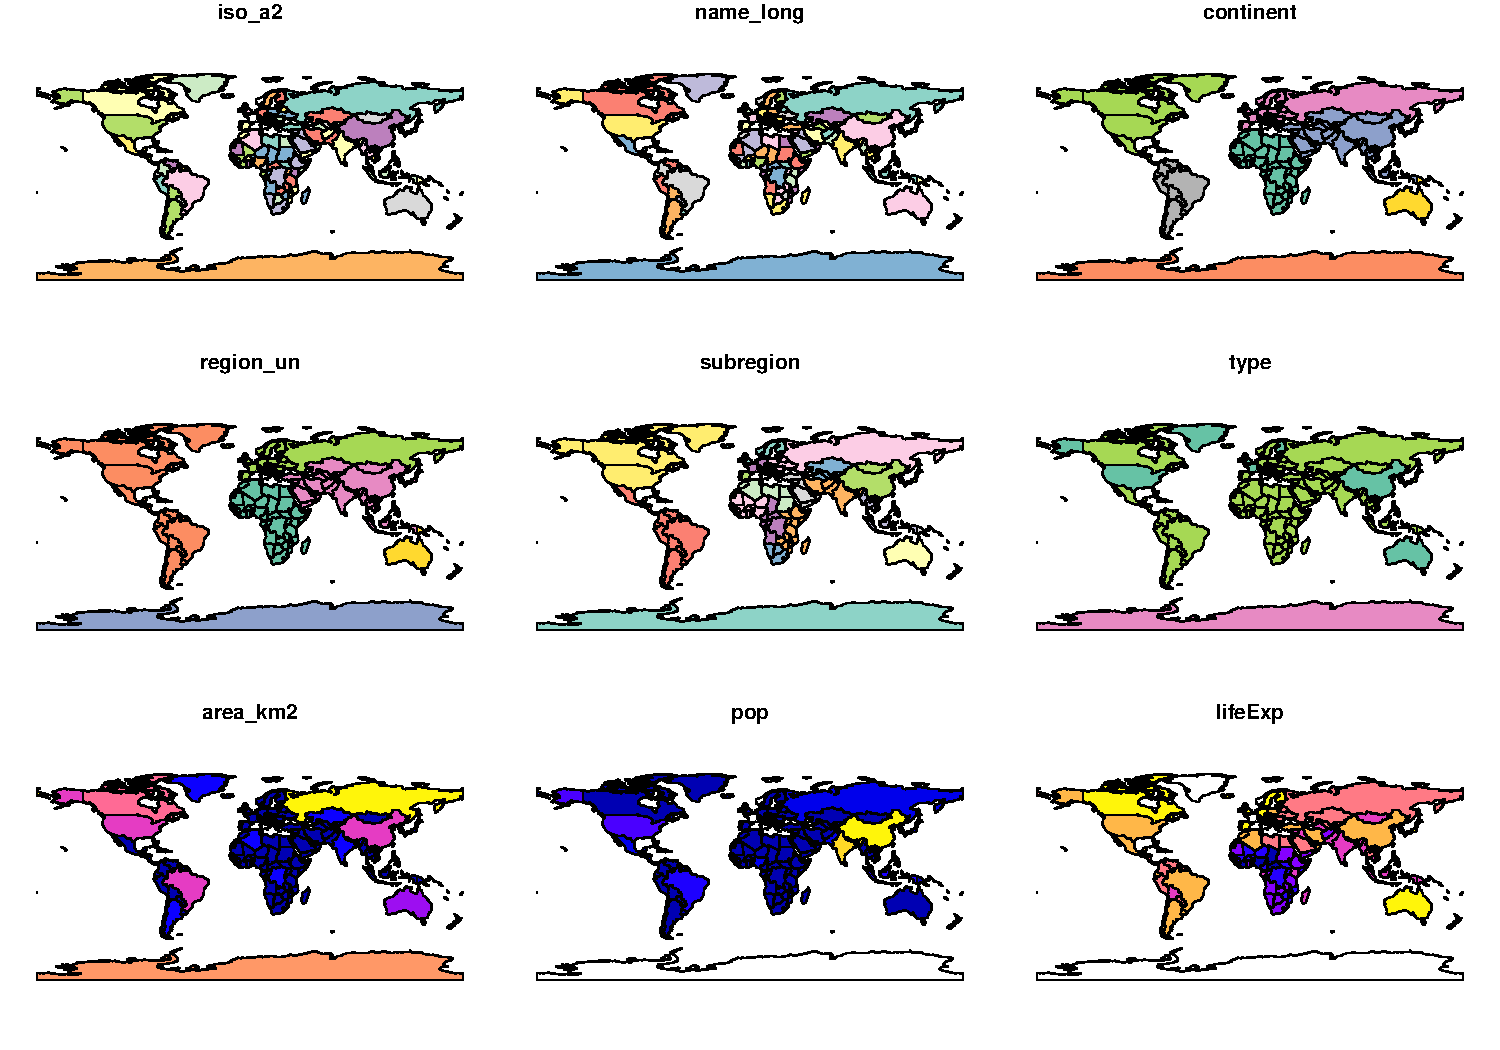
\includegraphics{A1_HalloWelt_files/figure-beamer/unnamed-chunk-19-1.pdf}

\end{frame}

\begin{frame}[fragile]{Nur einen Indikator plotten}

\begin{Shaded}
\begin{Highlighting}[]
\KeywordTok{plot}\NormalTok{(world[}\StringTok{"lifeExp"}\NormalTok{],}\DataTypeTok{main=}\StringTok{"Lebenserwartung in Jahren"}\NormalTok{)}
\end{Highlighting}
\end{Shaded}

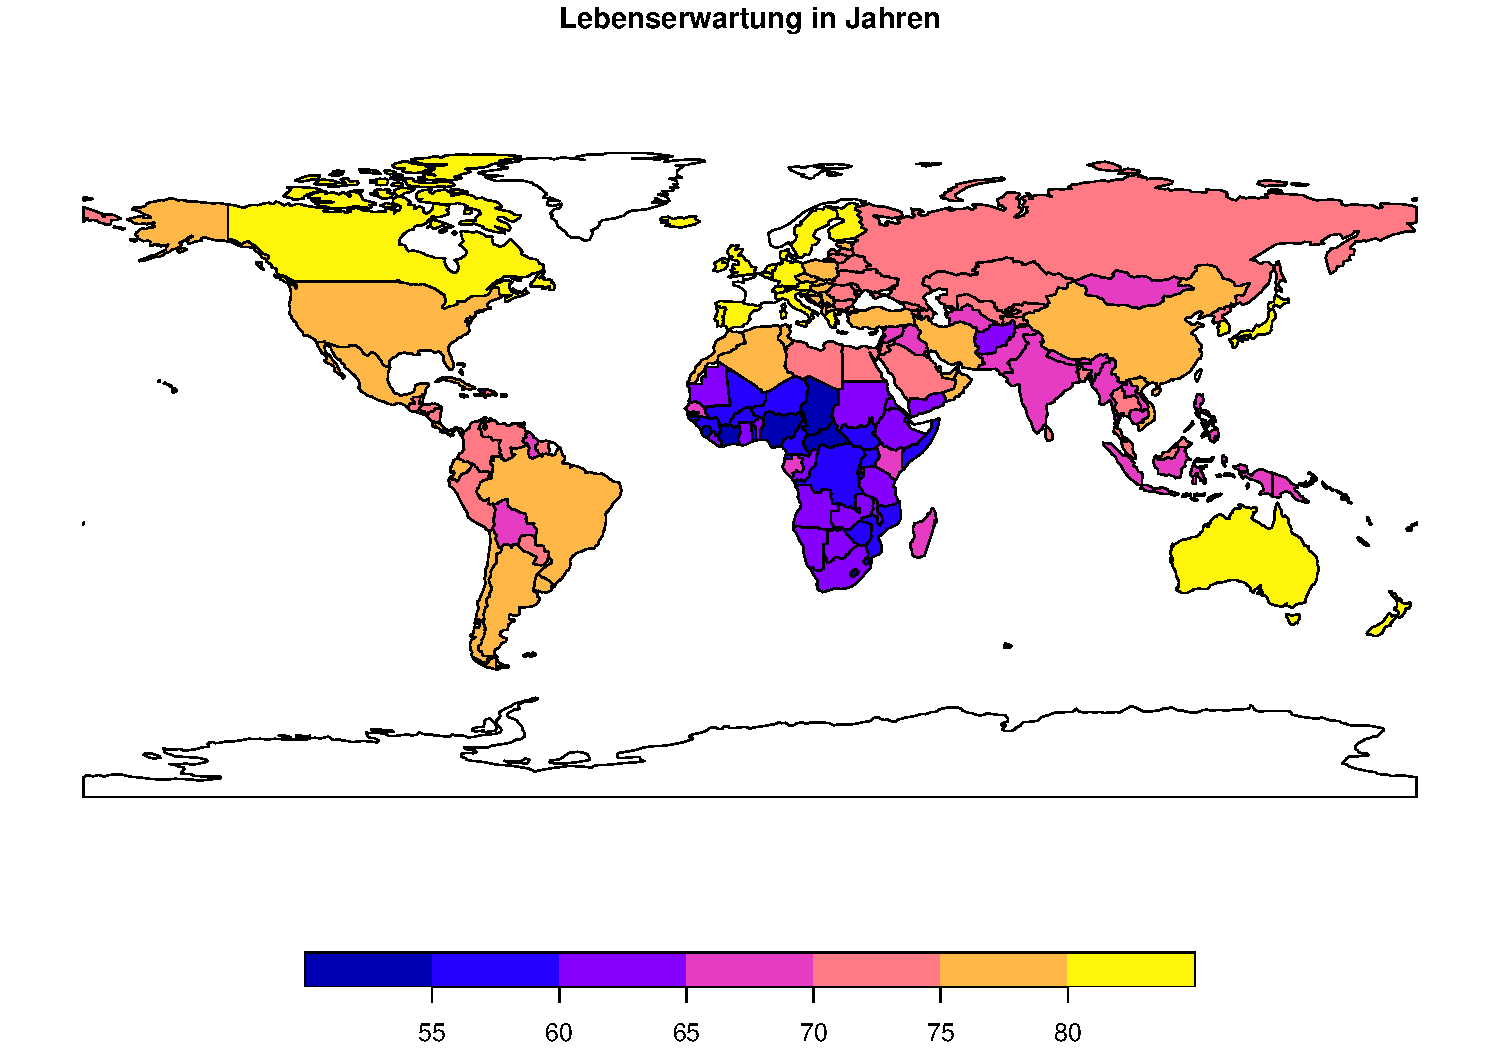
\includegraphics{A1_HalloWelt_files/figure-beamer/unnamed-chunk-20-1.pdf}

\end{frame}

\begin{frame}[fragile]{Eine andere Darstellungsform}

\begin{Shaded}
\begin{Highlighting}[]
 \KeywordTok{hist}\NormalTok{(world}\OperatorTok{$}\NormalTok{lifeExp,}\DataTypeTok{col=}\StringTok{"blue"}\NormalTok{,}\DataTypeTok{xlab=}\StringTok{"Lebenserwartung"}\NormalTok{,}
      \DataTypeTok{ylab=}\StringTok{"Häufigkeit"}\NormalTok{)}
\end{Highlighting}
\end{Shaded}

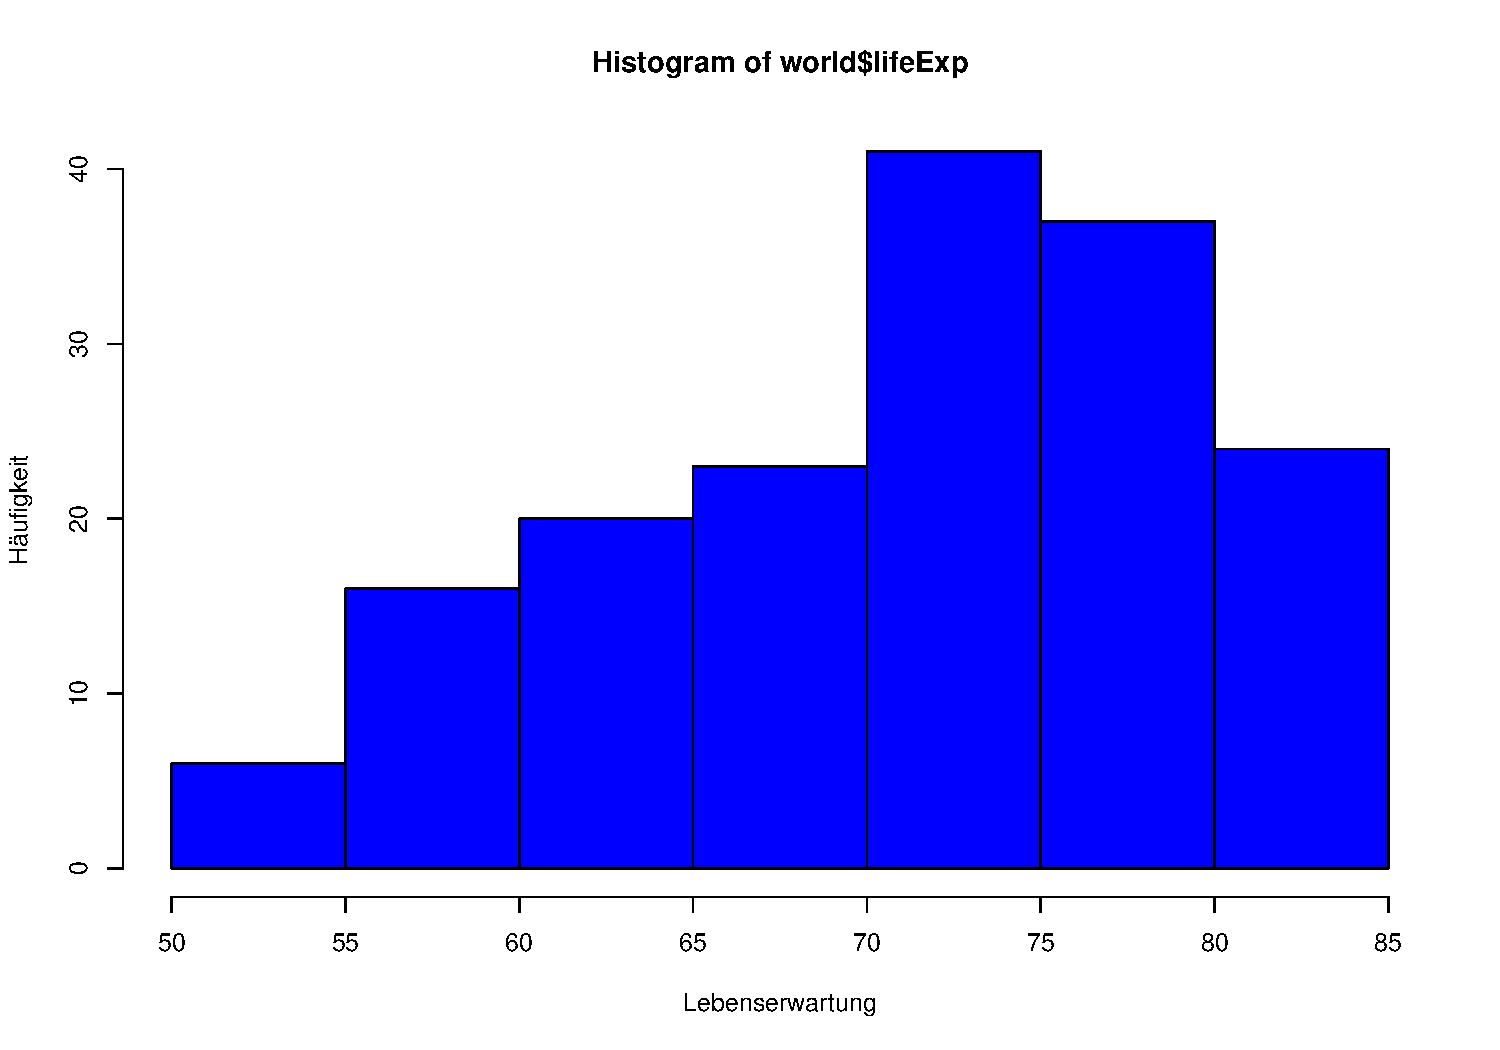
\includegraphics{A1_HalloWelt_files/figure-beamer/unnamed-chunk-21-1.pdf}

\end{frame}

\begin{frame}{\href{https://geocompr.robinlovelace.net/spatial-class.html}{Rasterdaten}}

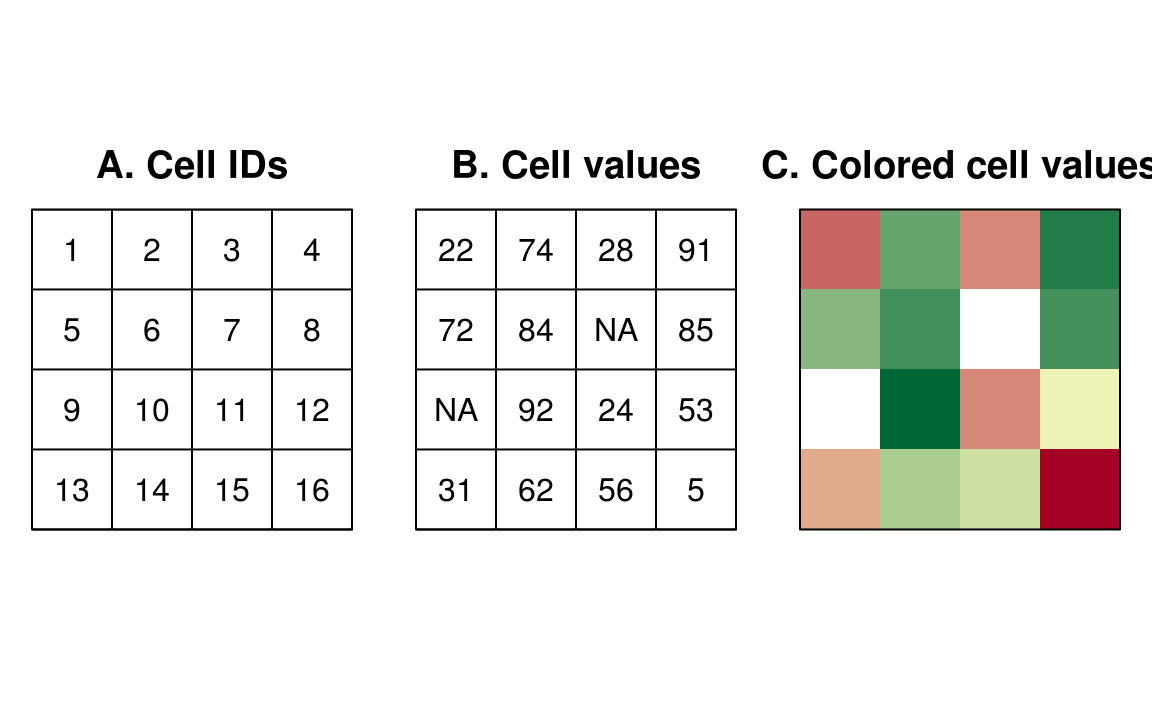
\includegraphics{figure/raster-intro-plot-1.png}

\end{frame}

\end{document}
